\svnidlong
{$HeadURL$}
{$LastChangedDate$}
{$LastChangedRevision$}
{$LastChangedBy$}
\svnid{$Id$}

Many different theories predict final states with a single top and associated missing 
transverse momentum (monotop), some of them including dark matter candidates. 
A simplified model encompassing the processes leading to this phenomenology is described in Refs.~\cite{AndreaFuksMaltoni,Agram:2013wda,Boucheneb:2014wza},
and is adopted as one of the benchmarks for Run 2 LHC searches. 

The simplified model is constructed by imposing that the model Lagrangian
respects the electroweak $SU(2)_L \times U(1)_Y$ gauge symmetry and by
requiring minimality in terms of new states to supplement to the Standard
Model fields. As a result, two monotop production mechanisms are possible.
In the first case, the monotop system is constituted by an invisible (or
long-lived with respect to detector distances) fermion $\chi$ and a top quark.
It is produced as shown in the diagram of \ref{fig:feyn_prod}~(a) where a colored
resonance $\varphi$ lying in the triplet representation of $SU(3)_C$ decays
into a top quark and a $\chi$ particle. In the second production mode, the
monotop state is made of a top quark and a vector state $V$ connected to a
hidden sector so that it could decay invisibly into, e.g., a pair of dark
matter particles as studied in~\cite{Boucheneb:2014wza}. The production proceeds via
flavor-changing neutral interactions of the top quark with a quark of the
first or second generation and the invisible $V$ boson (see the diagrams of
\ref{fig:feyn_prod}~(b) and (c)).

\begin{figure}[!h!tpd]
\centering
\unitlength=0.0046\textwidth
\subfloat[\label{subfig:S1}]{
  \begin{feynmandiagram}[modelS1]
    \fmfleft{i1,i2}
    \fmfright{o1,o2}
    \fmf{dashes,label={\Large $\varphi$}}{v1,v2}
    \fmf{fermion}{i2,v1,i1}
    \fmf{fermion}{v2,o1}
    \fmf{plain,tension=0}{v2,o2}
    \fmf{wiggly}{v2,o2}
    \fmfdot{v1,v2}
    \fmflabel{\Large ${\bar{s}}$}{i1}
    \fmflabel{\Large ${d}$}{i2}
    \fmflabel{\Large ${t}$}{o1}
    \fmflabel{\Large ${\chiDM}$}{o2}
  \end{feynmandiagram}
}\\\vspace{\baselineskip}
\subfloat[\label{subfig:S4s}]{
  \begin{feynmandiagram}[modelS4s]
    \fmfleft{i1,i2}
    \fmfright{o1,o2}
    \fmf{fermion,label={\LARGE $u$}}{v1,v2}
    \fmf{gluon}{i2,v1}
    \fmflabel{\LARGE $g$}{i2}
    \fmf{fermion}{i1,v1}
    \fmflabel{\LARGE $u$}{i1}
    \fmf{wiggly}{v2,o2}
    \fmf{fermion}{v2,o1}
    \fmflabel{\Large $V$}{o2}
    \fmflabel{\Large $t$}{o1}
  \end{feynmandiagram}
}
\subfloat[\label{subfig:S4t}]{
  \begin{feynmandiagram}[modelS4t]
    \fmfleft{i1,i2}
    \fmfright{o1,o2}
    \fmf{fermion}{i2,vup}
    \fmflabel{\LARGE $u$}{i2}
    \fmf{gluon}{i1,vdown}
    \fmflabel{\LARGE $g$}{i1}
    \fmf{fermion, label={\LARGE $t$}}{vup,vdown}
    \fmf{fermion}{vdown,o1}
    \fmflabel{\Large $t$}{o1}
    \fmf{wiggly}{vup,o2}
    \fmflabel{\Large $V$}{o2}
  \end{feynmandiagram}
  }
\caption
{
Feynman diagrams of leading order processes leading to monotop events: production of
a colored scalar resonance $\varphi$ decaying into a top quark and a spin-$1/2$ fermion $\chiDM$ (a),
$s-$ (b) and \tchannel (c) non resonant production of a top quark in association with
a spin-1 boson $V$ decaying invisibly.
}
\label{fig:feyn_prod}
\end{figure}


\newthought{Resonant production}
\label{sec:ResonantProd}

In this case, a colored $2/3$-charged scalar ($\varphi$) is produced and decays into a top quark and a spin-$1/2$ invisible particle, $\chiDM$.  The dynamics of the new sector is described by the following Lagrangian:
\be\label{eq:lagrangianResonant}\bsp
\lag  =
  \bigg[
    \varphi \bar d^c \Big[a^q_{SR} + b^q_{SR} \gamma_5 \Big] d +
    \varphi \bar u \Big[a^{1/2}_{SR} + b^{1/2}_{SR} \gamma_5 \Big] \chiDM
    +  {\rm h.c.} 
  \bigg] ,
\esp\ee
where $u$ ($d$) stands for any up-type (down-type) quark, the notation $SR$
refers to the monotop production mechanism via a scalar resonance and all
flavor and color indices are understood for clarity.

In the notation of~\cite{Agram:2013wda}, 
the couplings of the new colored fields to down-type quarks are
embedded into the $3\times 3$ antisymmetric matrices
$a^q_{SR}$ (scalar couplings) and $b^q_{SR}$ (pseudoscalar couplings)
while those to the new fermion $\chiDM$ and one
single up-type quark are given by the three-component vectors
$a^{1/2}_{S R}$ and $b^{1/2}_{S R}$
in flavor space. 


Under the form of Eq.~\eqref{eq:lagrangianResonant}, the Lagrangian is the one
introduced in the original monotop search proposal~\cite{AndreaFuksMaltoni}. It has been
used by the CMS collaboration for Run I analyses after neglecting all pseudoscalar components
of the couplings and adding the vector resonance case for which minimality
requirements are difficult to accommodate~\cite{Khachatryan:2014uma}. In contrast, the
study of Ref.~\cite{Boucheneb:2014wza} has imposed electroweak gauge invariance and
required minimality. This enforces all new couplings to be right-handed so that
\begin{equation}
a^{1/2}_{SR} = b^{1/2}_{SR} = \frac12 y_s^*
\qquad\text{and}\qquad
a^q_{SR} = b^q_{SR} = \frac12 \lambda_s \ ,
\end{equation}
where the objects $y_s$ and $\lambda_s$ are
a tridimensional vector and a $3\times 3$ matrix
in flavor space respectively. 
This class of scenarios is the one that has been adopted by the ATLAS collaboration for its
Run~I monotop searches~\cite{Aad:2014wza} and will be considered by both
collaborations for Run~II analyses.

The resulting model can be likened to the MSSM with an $R$-parity violating of
a top squark to the Standard Model down-type quarks and an $R$-parity
conserving interaction of a top quark and a top-squark to a neutralino.
  

\newthought{Non-Resonant production}
\label{sec:NonResonantProd}

For non-resonant monotop production, the monotop state is produced via
flavor-changing neutral interactions of the top quark, a lighter up-type
quark and a new invisible vector particle $V$. 
This is the only case considered, as having a new scalar 
would involve in particular a mixing with the SM Higgs boson and therefore a larger number of free parameters. 
The Lagrangian describing the
dynamics of this non-resonant monotop production case is:
\be\label{eq:lagrangianNonResonantVector}\bsp
\lag =
  \bigg[
    V_\mu \bar u \gmu \Big[a^1_{FC} \!+\! b^1_{FC} \gamma_5 \Big] u  
    + \rm h.c. 
  \bigg] \ ,
\esp\ee
where the flavor and color indices are
again understood for clarity.
The strength of the interactions among these two states and a pair
of up-type quarks is modeled via two $3\times 3$ matrices in flavor space $a^{1}_{FC}$ for the vector couplings
and $b^{1}_{FC}$ for the axial vector couplings, the $FC$ subscript referring to the flavor-changing neutral
monotop production mode and the $(1)$ superscript to the vectorial nature of the invisible particle.

As for the resonant case, the Lagrangian of Eq.~\eqref{eq:lagrangianNonResonantVector} is the one that
has been used by CMS after reintroducing the scalar option for the invisible
state and neglecting all pseudoscalar interactions~\cite{Khachatryan:2014uma}. As
already mentioned, a simplified setup motivated by gauge invariance and
minimality has been preferred so that, as shown in Ref.~\cite{Boucheneb:2014wza}, we
impose all interactions to involve right-handed quarks only,
\begin{equation}
a^1_{FC} = b^1_{FC} = \frac12 a_R
\end{equation}
where $a_R$ denotes a $3\times 3$ matrix in flavor space.
This implies the vector field to be an $SU(2)_L$
singlet.

\newthought{Model parameters and assumptions}
 
The models considered as benchmarks for the first LHC searches
contain further assumptions in terms of the flavor structure of the model
with respect to the Lagrangians of the previous subsection.
In order to have an observable monotop signature at the LHC, the Lagrangians
introduced above must include not too small couplings of the new particles to
first and second generation quarks. For simplicity, we assumed that only
channels enhanced by parton density effects will be considered, so that we fix
\begin{equation}\bsp
(a_R)_{13} = (a_R)_{31} = a \ , \\
(\lambda_s)_{12} = - (\lambda_s)_{21} = \lambda
\qquad\text{and}\qquad
(y_s)_3 = y \ ,
\esp\end{equation}
all other elements of the matrices and vectors above being set to zero.

%\Todo{There is still an on-going study that should be finished very soon (by the end
%	of the week). The point is that CMS is fixing the $y$ parameters in the way that
%	the branching ratio of the scalar resonance into a monotop system is close to
%	100\%, while ATLAS is fixing y = lambda. We are investigating both cases so to
%	conclude whether this is good to keep both options allowed.
%	}


\newthought{Implementation}
     In order to allow one for the Monte Carlo simulation of events relevant for
     the monotop production cases described above, we consider the Lagrangian
     \be
       \lag =
         \bigg[
             a V_\mu \bar u \gmu P_R t
           + \lambda \varphi \bar d^c P_R s
           + y \varphi \bar \chiDM P_R t
           +  {\rm h.c.} \ ,
         \bigg]
     \ee
     where $P_R$ stands for the right-handed chirality projector and the new
     physics couplings are defined by the three parameters $a$, $\lambda$ and
     $y$. We additionally include a coupling of the invisible vector boson $V$
     to a dark sector (represented by a fermion $\psi$) whose strength can be
     controlled through a parameter $g_{DM}$,
     \be
       \lag = g_{DM} V_\mu \bar\psi \gamma^\mu\psi \ .
     \ee
     This ensures the option to make the $V$-boson effectively invisible by
     tuning $g_{DM}$ respectively to $a$. We implement the entire model in the
     {\sc FeynRules} package~\cite{Alloul:2013bka} so that the model can be
     exported to a UFO library~\cite{Degrande:2011ua} to be linked to
     {\sc MadGraph5\_aMC@NLO}~\cite{Alwall:2014hca} for event generation,
     following the approach outlined in~\cite{Christensen:2009jx}.


\subsection{Parameter scan}

Under all the assumptions of the previous sections, the parameter space of
the resonant model is defined by four quantities, namely the mass of the
new scalar field $\varphi$, the mass of the invisible fermion $\chi$ and
the strengths of the interactions of the scalar resonance with the monotop
system $y$ and with down-type quarks $\lambda$. One of both coupling
parameters could however be traded with the width of the resonance.

The parameter space of the non-resonant model is defined by two
parameters, namely the mass of the invisible state $V$ and its
flavor-changing neutral coupling to the up-type quarks $a_R$.

In the case of the non-resonant model, the invisible vector is connected to
a hidden sector that could be, in its simplest form, parameterized by a new
fermion~\cite{Boucheneb:2014wza}. This has effects on the width of the invisible $V$ state.


A consensus between the ATLAS and CMS collaborations has been reached in
the case of non-resonant monotop production. The results have been
described above. In contrast, discussions in the context of resonant
monotop production are still on-going. The related parameter space
contains four parameters and must thus be further simplified for practical
purposes. Several options are possible and a choice necessitates additional
studies that will be achieved in a near future.



It has been verified that the kinematics do not depend on the width of the
invisible state in the case where this width is at most 10\% of the
$V$-mass. This is illustrated in Figures~\ref{fig:appB:Vmass} and \ref{fig:appB:pTV},
where we respectively show the invariant-mass and transverse-momentum
spectra of the $V$-boson when it decays into a top-up final state and for
different $V$-boson masses. The results are however independent of the
visible or invisible decay modes as we are only concerned with the
kinematical properties of the invisible state.

\begin{figure}[!h!tpd]
	\centering
	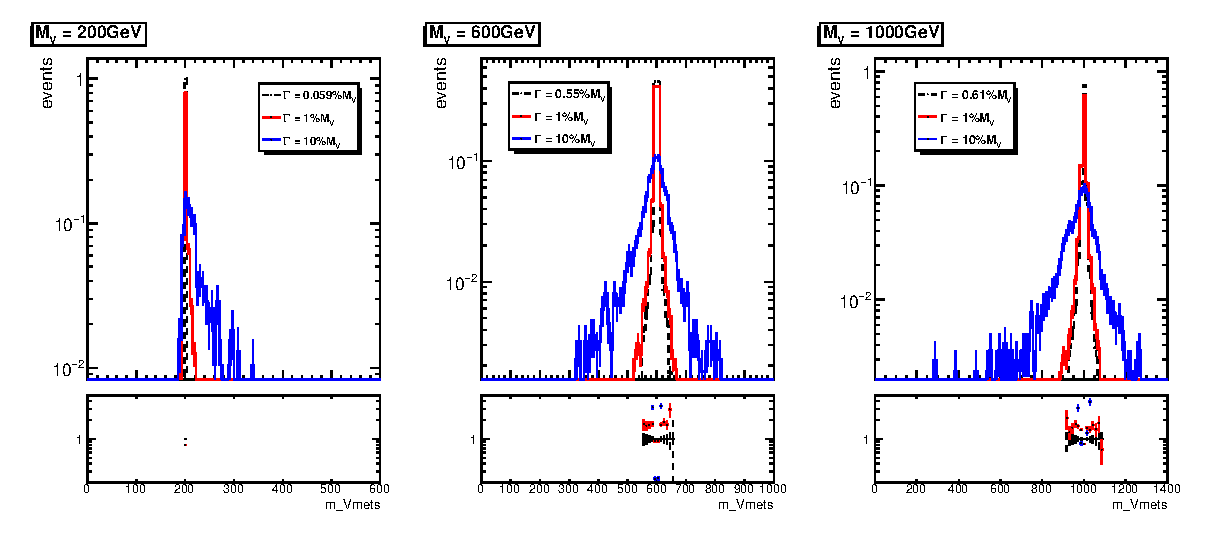
\includegraphics[width=1.0\textwidth]{figures/singletop/m_Vmets}
	\caption{
Distributions of the invariant mass of the $V$ boson in the case of
the process $p p \to tV \to t (t\bar u + {\rm c.c.})$. We have imposed
that the $V$-boson is produced on-shell and have chosen its mass to be
$m_V = 200$, 600 and 1000~GeV (left, central and right panels).
Moreover, we have considered three possible cases for the total width
of the $V$-boson, which has been fixed to 0.61\%, 0.1\% and 10\% of the
mass.
}   
	\label{fig:appB:Vmass}
\end{figure}


\begin{figure}[!h!tpd]
	\centering
	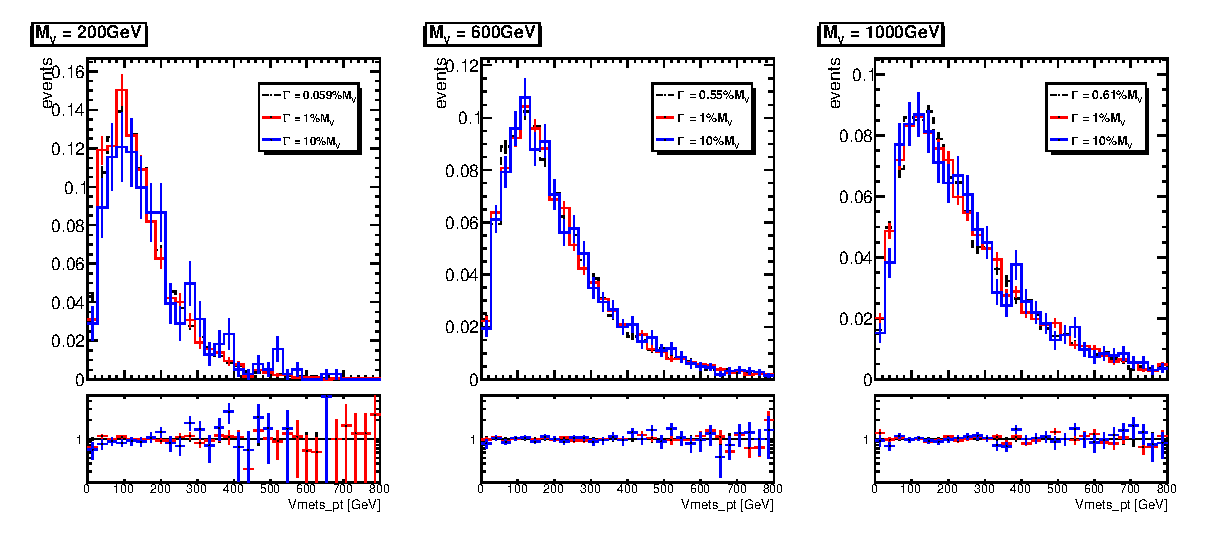
\includegraphics[width=1.0\textwidth]{figures/singletop/Vmets_pt}
	\caption{
Same as Figure~\ref{fig:appB:Vmass} in the case of the transverse-momentum
distribution of the $V$-boson.
	}
	\label{fig:appB:pTV}
\end{figure}


\subsection{Single Top Models}
  Card files for \madgraph are provided on the Forum SVN
  repository~\cite{ForumSVN_EWMonoTop} and correspond to the Lagrangian that has
  been implemented in {\sc FeynRules}. Each coupling constant of the model can
  be set via the block \texttt{COUPX} of the parameter card. Its entries 1, 2
  and 3 respectively correspond to the monotop-relevant parameters $a$,
  $\lambda$ and $y$, while the width (and in particular the invisible partial
  width) of the $V$-boson can be tuned {\it via} the $g_{DM}$ parameter to given
  in the entry 10 of the \texttt{COUPX} block.

  The masses of the particles are set in the \texttt{MASS} block of the
  parameter card, the PDG codes of the new states being 32 (the vector state
  $V$), 1000006 (the $\varphi$ colored resonance), 1000022 (the invisible fermion
  $\chiDM$) and 1000023 (the fermion $\psi$ connecting the $V$ state to the dark
  sector). The width of the new vector has to be computed from all open
  tree-level decays (after fixing $g_{DM}$ to a large value and setting the
  relevant entry to \texttt{Auto} in the \texttt{DECAY} block of the parameter
  card), while the way to calculate the width of the resonance $\phi$ is under
  discussion by both the ATLAS and CMS collaborations. The $chi$ and $psi$
  fermions are taken stable so that their width vanishes.
